\chapterimage{chapter_head_1.pdf}
\chapter{Tuples}
\label{tuplechap}

\section{Tuples are immutable}

\index{tuple}
\index{type!tuple}
\index{sequence}

A tuple is a sequence of values.  The values can be any type, and
they are indexed by integers, so in that respect tuples are a lot
like lists.  The important difference is that tuples are immutable.
%
\index{mutability}
\index{immutability}
%
Syntactically, a tuple is a comma-separated list of values:

\beforeverb
\begin{pycode}
>>> t = 'a', 'b', 'c', 'd', 'e'
\end{pycode}
\afterverb
%
Although it is not necessary, it is common to enclose tuples in
parentheses:

\index{parentheses!tuples in}

\beforeverb
\begin{pycode}
>>> t = ('a', 'b', 'c', 'd', 'e')
\end{pycode}
\afterverb
%
To create a tuple with a single element, you have to include a final
comma:

\index{singleton}
\index{tuple!singleton}

\beforeverb
\begin{pycode}
>>> t1 = ('a',)
>>> type(t1)
<type 'tuple'>
\end{pycode}
\afterverb
%
A value in parentheses is not a tuple:

\beforeverb
\begin{pycode}
>>> t2 = ('a')
>>> type(t2)
<type 'str'>
\end{pycode}
\afterverb
%
Another way to create a tuple is the built-in function {\tt tuple}.
With no argument, it creates an empty tuple:

\index{tuple function}
\index{function!tuple}

\beforeverb
\begin{pycode}
>>> t = tuple()
>>> print(t)
()
\end{pycode}
\afterverb
%
If the argument is a sequence (string, list or tuple), the result
is a tuple with the elements of the sequence:

\beforeverb
\begin{pycode}
>>> t = tuple('lupins')
>>> print(t)
('l', 'u', 'p', 'i', 'n', 's')
\end{pycode}
\afterverb
%
Because {\tt tuple} is the name of a built-in function, you should
avoid using it as a variable name.
Most list operators also work on tuples.  The bracket operator
indexes an element:

\index{bracket operator}
\index{operator!bracket}

\beforeverb
\begin{pycode}
>>> t = ('a', 'b', 'c', 'd', 'e')
>>> print(t[0])
'a'
\end{pycode}
\afterverb
%
And the slice operator selects a range of elements.

\index{slice operator}
\index{operator!slice}
\index{tuple!slice}
\index{slice!tuple}

\beforeverb
\begin{pycode*}{firstnumber = last}
>>> print(t[1:3])
('b', 'c')
\end{pycode*}
\afterverb
%
But if you try to modify one of the elements of the tuple, you get
an error:

\index{exception!TypeError}
\index{TypeError}
\index{item assignment}
\index{assignment!item}

\beforeverb
\begin{pycode*}{firstnumber = last}
>>> t[0] = 'A'
TypeError: object doesn't support item assignment
\end{pycode*}
\afterverb
%
You can't modify the elements of a tuple, but you can replace
one tuple with another:

\beforeverb
\begin{pycode*}{firstnumber = last}
>>> t = ('A',) + t[1:]
>>> print(t)
('A', 'b', 'c', 'd', 'e')
\end{pycode*}
\afterverb
%

\section{Tuple assignment}
\label{tuple assignment}

\index{tuple!assignment}
\index{assignment!tuple}
\index{swap pattern}
\index{pattern!swap}

It is often useful to swap the values of two variables.
With conventional assignments, you have to use a temporary
variable.  For example, to swap {\tt a} and {\tt b}:

\beforeverb
\begin{pycode}
>>> temp = a
>>> a = b
>>> b = temp
\end{pycode}
\afterverb
%
This solution is cumbersome; {\bf tuple assignment} is more elegant:

\beforeverb
\begin{pycode}
>>> a, b = b, a
\end{pycode}
\afterverb
%
The left side is a tuple of variables; the right side is a tuple of
expressions.  Each value is assigned to its respective variable.  
All the expressions on the right side are evaluated before any
of the assignments.
%
The number of variables on the left and the number of
values on the right have to be the same:

\index{exception!ValueError}
\index{ValueError}

\beforeverb
\begin{pycode}
>>> a, b = 1, 2, 3
ValueError: too many values to unpack
\end{pycode}
\afterverb
%
More generally, the right side can be any kind of sequence
(string, list or tuple).  For example, to split an email address
into a user name and a domain, you could write:

\index{split method}
\index{method!split}
\index{email address}

\beforeverb
\begin{pycode}
>>> addr = 'monty@python.org'
>>> uname, domain = addr.split('@')
\end{pycode}
\afterverb
%
The return value from {\tt split} is a list with two elements;
the first element is assigned to {\tt uname}, the second to
{\tt domain}.

\beforeverb
\begin{pycode*}{firstnumber = last}
>>> print(uname)
monty
>>> print(domain)
python.org
\end{pycode*}
\afterverb
%

\section{Tuples as return values}

\index{tuple}
\index{value!tuple}
\index{return value!tuple}
\index{function, tuple as return value}

Strictly speaking, a function can only return one value, but
if the value is a tuple, the effect is the same as returning
multiple values.  For example, if you want to divide two integers
and compute the quotient and remainder, it is inefficient to
compute {\tt x/y} and then {\tt x\%y}.  It is better to compute
them both at the same time.
%
\index{divmod}
%
The built-in function {\tt divmod} takes two arguments and
returns a tuple of two values, the quotient and remainder.
You can store the result as a tuple:

\beforeverb
\begin{pycode}
>>> t = divmod(7, 3)
>>> print(t)
(2, 1)
\end{pycode}
\afterverb
%
Or use tuple assignment to store the elements separately:

\index{tuple assignment}
\index{assignment!tuple}

\beforeverb
\begin{pycode}
>>> quot, rem = divmod(7, 3)
>>> print(quot)
2
>>> print(rem)
1
\end{pycode}
\afterverb
%
Here is an example of a function that returns a tuple:

\beforeverb
\begin{pycode}
def min_max(t):
    return min(t), max(t)
\end{pycode}
\afterverb
%
{\tt max} and {\tt min} are built-in functions that find
the largest and smallest elements of a sequence.  \verb"min_max"
computes both and returns a tuple of two values.

\index{max function}
\index{function!max}
\index{min function}
\index{function!min}


\section{Variable-length argument tuples}

\index{variable-length argument tuple}
\index{argument!variable-length tuple}
\index{gather}
\index{parameter!gather}
\index{argument!gather}

Functions can take a variable number of arguments.  A parameter
name that begins with {\tt *} {\bf gathers} arguments into
a tuple.  For example, {\tt printall}
takes any number of arguments and prints them:

\beforeverb
\begin{pycode}
def printall(*args):
    print(args)
\end{pycode}
\afterverb
%
The gather parameter can have any name you like, but {\tt args} is
conventional.  Here's how the function works:

\beforeverb
\begin{pycode}
>>> printall(1, 2.0, '3')
(1, 2.0, '3')
\end{pycode}
\afterverb
%
The complement of gather is {\bf scatter}.  If you have a
sequence of values and you want to pass it to a function
as multiple arguments, you can use the {\tt *} operator.
For example, {\tt divmod} takes exactly two arguments; it
doesn't work with a tuple:

% removing this because we haven't seen optional parameters yet
%You can combine the gather operator with required and positional
%arguments:

%\beforeverb
%\begin{pycode}
%def pointless(required, optional=0, *args):
%    print required, optional, args
%\end{pycode}
%\afterverb
%
%Run this function with 1, 2, 3 and 4 or more arguments and
%make sure you understand what it does.

\index{scatter}
\index{argument scatter}

\index{TypeError}
\index{exception!TypeError}

\beforeverb
\begin{pycode}
>>> t = (7, 3)
>>> divmod(t)
TypeError: divmod expected 2 arguments, got 1
\end{pycode}
\afterverb
%
But if you scatter the tuple, it works:

\beforeverb
\begin{pycode}
>>> divmod(*t)
(2, 1)
\end{pycode}
\afterverb
%
\begin{exercise}
Many of the built-in functions use
variable-length argument tuples.  For example, {\tt max}
and {\tt min} can take any number of arguments:

\index{max function}
\index{function!max}
\index{min function}
\index{function!min}

\beforeverb
\begin{pyexo}
>>> max(1,2,3)
3
\end{pyexo}
\afterverb
%
But {\tt sum} does not.

\index{sum function}
\index{function!sum}

\beforeverb
\begin{pyexo}
>>> sum(1,2,3)
TypeError: sum expected at most 2 arguments, got 3
\end{pyexo}
\afterverb
%
Write a function called {\tt sumall} that takes any number
of arguments and returns their sum.

\end{exercise}

\section{Lists and tuples}
\begin{color}{red}

\index{zip function}
\index{function!zip}

{\tt zip} is a built-in function that takes two or more sequences and
``zips'' them into a list\footnote{In Python 3.0, {\tt zip} returns an
  iterator of tuples, but for most purposes, an iterator behaves like
  a list.} of tuples where each tuple contains one element from each
sequence.

\index{Python 3.0}

This example zips a string and a list:

\beforeverb
\begin{pycode}
>>> s = 'abc'
>>> t = [0, 1, 2]
>>> zip(s, t)
[('a', 0), ('b', 1), ('c', 2)]
\end{pycode}
\afterverb
%
The result is a list of tuples where each tuple contains
a character from the string and the corresponding element from
the list.

\index{list!of tuples}

If the sequences are not the same length, the result has the
length of the shorter one.

\beforeverb
\begin{pycode}
>>> zip('Anne', 'Elk')
[('A', 'E'), ('n', 'l'), ('n', 'k')]
\end{pycode}
\afterverb

\end{color}
%
You can use tuple assignment in a {\tt for} loop to traverse a list of
tuples:

\index{traversal}
\index{tuple assignment}
\index{assignment!tuple}

\beforeverb
\begin{pycode}
t = [('a', 0), ('b', 1), ('c', 2)]
for letter, number in t:
    print(number, letter)
\end{pycode}
\afterverb
%
Each time through the loop, Python selects the next tuple in
the list and assigns the elements to {\tt letter} and 
{\tt number}.  The output of this loop is:

\index{loop}

\beforeverb
\begin{pyoutput}
0 a
1 b
2 c
\end{pyoutput}
\afterverb
%
If you combine {\tt zip}, {\tt for} and tuple assignment, you get a
useful idiom for traversing two (or more) sequences at the same
time.  For example, \verb"has_match" takes two sequences, {\tt t1} and
{\tt t2}, and returns {\tt True} if there is an index {\tt i}
such that {\tt t1[i] == t2[i]}:

\index{for loop}

\beforeverb
\begin{pycode}
def has_match(t1, t2):
    for x, y in zip(t1, t2):
        if x == y:
            return True
    return False
\end{pycode}
\afterverb
%
If you need to traverse the elements of a sequence and their
indices, you can use the built-in function {\tt enumerate}:

\index{traversal}
\index{enumerate function}
\index{function!enumerate}

\beforeverb
\begin{pycode}
for index, element in enumerate('abc'):
    print(index, element)
\end{pycode}
\afterverb
%
The output of this loop is:

\beforeverb
\begin{pyoutput}
0 a
1 b
2 c
\end{pyoutput}
\afterverb
%
Again.


\section{Dictionaries and tuples}

\index{dictionary}
\index{items method}
\index{method!items}
\index{key-value pair}

Dictionaries have a method called {\tt items} that returns a list of
tuples, where each tuple is a key-value pair\footnote{This behavior is
  slightly different in Python 3.0.}.

\beforeverb
\begin{pycode}
>>> d = {'a':0, 'b':1, 'c':2}
>>> t = d.items()
>>> print(t)
[('a', 0), ('c', 2), ('b', 1)]
\end{pycode}
\afterverb
%
As you should expect from a dictionary, the items are in no
particular order.

\index{dictionary!initialize}

Conversely, you can use a list of tuples to initialize
a new dictionary:

\beforeverb
\begin{pycode}
>>> t = [('a', 0), ('c', 2), ('b', 1)]
>>> d = dict(t)
>>> print(d)
{'a': 0, 'c': 2, 'b': 1}
\end{pycode}
\afterverb

Combining {\tt dict} with {\tt zip} yields a concise way
to create a dictionary:

\index{zip function!use with dict}

\beforeverb
\begin{pycode}
>>> d = dict(zip('abc', range(3)))
>>> print(d)
{'a': 0, 'c': 2, 'b': 1}
\end{pycode}
\afterverb
%
The dictionary method {\tt update} also takes a list of tuples
and adds them, as key-value pairs, to an existing dictionary.

\index{update method}
\index{method!update}

\index{traverse!dictionary}
\index{dictionary!traversal}

Combining {\tt items}, tuple assignment and {\tt for}, you
get the idiom for traversing the keys and values of a dictionary:

\beforeverb
\begin{pycode}
for key, val in d.items():
    print(val, key)
\end{pycode}
\afterverb
%
The output of this loop is:

\beforeverb
\begin{pyoutput}
0 a
2 c
1 b
\end{pyoutput}
\afterverb
%
Again.

\index{tuple!as key in dictionary}
\index{hashable}

It is common to use tuples as keys in dictionaries (primarily because
you can't use lists).  For example, a telephone directory might map
from last-name, first-name pairs to telephone numbers.  Assuming
that we have defined {\tt last}, {\tt first} and {\tt number}, we
could write:

\beforeverb
\begin{pycode}
directory[(last,first)] = number
\end{pycode}
\afterverb
%
The expression in brackets is a tuple.  We could use tuple
assignment to traverse this dictionary.

\index{tuple!in brackets}

\beforeverb
\begin{pycode}
for last, first in directory:
    print(first, last, directory[(last,first)])
\end{pycode}
\afterverb
%
This loop traverses the keys in {\tt directory}, which are tuples.  It
assigns the elements of each tuple to {\tt last} and {\tt first}, then
prints the name and corresponding telephone number.

There are two ways to represent tuples in a state diagram.  The more
detailed version shows the indices and elements just as they appear in
a list.  For example, the tuple \verb"('Cleese', 'John')" would appear:

\index{state diagram}
\index{diagram!state}

\beforefig
\centerline{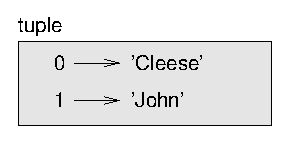
\includegraphics{figs/tuple1.eps}}
\afterfig

But in a larger diagram you might want to leave out the
details.  For example, a diagram of the telephone directory might
appear:

\beforefig
\centerline{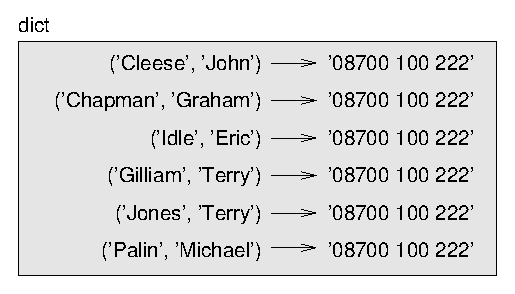
\includegraphics{figs/dict2.eps}}
\afterfig

Here the tuples are shown using Python syntax as a graphical
shorthand.
%
The telephone number in the diagram is the complaints line for the
BBC, so please don't call it.



\section{Comparing tuples}

\index{comparison!tuple}
\index{tuple!comparison}
\index{sort method}
\index{method!sort}

The relational operators work with tuples and other sequences;
Python starts by comparing the first element from each
sequence.  If they are equal, it goes on to the next elements,
and so on, until it finds elements that differ.  Subsequent
elements are not considered (even if they are really big).

\beforeverb
\begin{pycode}
>>> (0, 1, 2) < (0, 3, 4)
True
>>> (0, 1, 2000000) < (0, 3, 4)
True
\end{pycode}
\afterverb
%
The {\tt sort} function works the same way.  It sorts 
primarily by first element, but in the case of a tie, it sorts
by second element, and so on.  
%
This feature lends itself to a pattern called {\bf DSU} for 

\begin{description}

\item[Decorate] a sequence by building a list of tuples
with one or more sort keys preceding the elements from the sequence,

\item[Sort] the list of tuples, and

\item[Undecorate] by extracting the sorted elements of the sequence.

\end{description}

\label{DSU}
\index{DSU pattern}
\index{pattern!DSU}
\index{decorate-sort-undecorate pattern}
\index{pattern!decorate-sort-undecorate}

For example, suppose you have a list of words and you want to
sort them from longest to shortest:

\beforeverb
\begin{pycode}
def sort_by_length(words):
    t = []
    for word in words:
       t.append((len(word), word))

    t.sort(reverse=True)

    res = []
    for length, word in t:
        res.append(word)
    return res
\end{pycode}
\afterverb
%
The first loop builds a list of tuples, where each
tuple is a word preceded by its length.
%
{\tt sort} compares the first element, length, first, and
only considers the second element to break ties.  The keyword argument
{\tt reverse=True} tells {\tt sort} to go in decreasing order.
%
\index{keyword argument}
\index{argument!keyword}
\index{traversal}
%
The second loop traverses the list of tuples and builds a list of
words in descending order of length.

\begin{exercise}
In this example, ties are broken by comparing words, so words
with the same length appear in reverse alphabetical order.  For other
applications you might want to break ties at random.  Modify
this example so that words with the same length appear in
random order.  Hint: see the {\tt random} function in the
{\tt random} module.

\index{random module}
\index{module!random}
\index{random function}
\index{function!random}

\end{exercise}


\section{Sequences of sequences}
\index{sequence}

I have focused on lists of tuples, but almost all of the examples in
this chapter also work with lists of lists, tuples of tuples, and
tuples of lists.  To avoid enumerating the possible combinations, it
is sometimes easier to talk about sequences of sequences.
%
In many contexts, the different kinds of sequences (strings, lists and
tuples) can be used interchangeably.  So how and why do you choose one
over the others?

\index{string}
\index{list}
\index{tuple}
\index{mutability}
\index{immutability}

To start with the obvious, strings are more limited than other
sequences because the elements have to be characters.  They are
also immutable.  If you need the ability to change the characters
in a string (as opposed to creating a new string), you might
want to use a list of characters instead.

Lists are more common than tuples, mostly because they are mutable.
But there are a few cases where you might prefer tuples:

\begin{enumerate}

\item In some contexts, like a {\tt return} statement, it is
syntactically simpler to create a tuple than a list.  In other
contexts, you might prefer a list.

\item If you want to use a sequence as a dictionary key, you
have to use an immutable type like a tuple or string.

\item If you are passing a sequence as an argument to a function,
using tuples reduces the potential for unexpected behavior
due to aliasing.

\end{enumerate}

Because tuples are immutable, they don't provide methods
like {\tt sort} and {\tt reverse}, which modify existing lists.
But Python provides the built-in functions {\tt sorted}
and {\tt reversed}, which take any sequence as a parameter
and return a new list with the same elements in a different
order.

\index{sorted function}
\index{function!sorted}
\index{reversed function}
\index{function!reversed}


\section{Glossary}
	
\begin{vocabulary}[tuple:] An immutable sequence of elements.
\index{tuple}
\end{vocabulary}
	
\begin{vocabulary}[tuple assignment:] An assignment with a sequence on the
right side and a tuple of variables on the left.  The right
side is evaluated and then its elements are assigned to the
variables on the left.
\index{tuple assignment}
\index{assignment!tuple}
\end{vocabulary}
	
\begin{vocabulary}[gather:] The operation of assembling a variable-length
argument tuple.
\index{gather}
\end{vocabulary}
	
\begin{vocabulary}[scatter:] The operation of treating a sequence as a list of
arguments.
\index{scatter}
\end{vocabulary}
	
\begin{vocabulary}[DSU:] Abbreviation of ``decorate-sort-undecorate,'' a
pattern that involves building a list of tuples, sorting, and
extracting part of the result.
\index{DSU pattern}
\end{vocabulary}
	
\begin{vocabulary}[data structure:] A collection of related values, often
organized in lists, dictionaries, tuples, etc.
\index{data structure}
\end{vocabulary}
	
\begin{vocabulary}[shape (of a data structure):] A summary of the type,
size and composition of a data structure.
\index{shape}
\end{vocabulary}
	


\section{Exercises}

\begin{exercise}
Write a function called \verb"most_frequent" that takes a string and
prints the letters in decreasing order of frequency.  Find text
samples from several different languages and see how letter frequency
varies between languages.  Compare your results with the tables at
\url{wikipedia.org/wiki/Letter_frequencies}.

\index{letter frequency}
\index{frequency!letter}

\end{exercise}


\begin{exercise}
\label{anagrams}

\index{anagram set}
\index{set!anagram}

More anagrams!

\begin{enumerate}

\item Write a program
that reads a word list from a file (see Section~\ref{wordlist}) and
prints all the sets of words that are anagrams.

Here is an example of what the output might look like:

\beforeverb
\begin{pyexo}
['deltas', 'desalt', 'lasted', 'salted', 'slated', 'staled']
['retainers', 'ternaries']
['generating', 'greatening']
['resmelts', 'smelters', 'termless']
\end{pyexo}
\afterverb
%
Hint: you might want to build a dictionary that maps from a
set of letters to a list of words that can be spelled with those
letters.  The question is, how can you represent the set of
letters in a way that can be used as a key?

\item Modify the previous program so that it prints the largest set
of anagrams first, followed by the second largest set, and so on.

\index{Scrabble}
\index{bingo}

\item In Scrabble a ``bingo'' is when you play all seven tiles in
your rack, along with a letter on the board, to form an eight-letter
word.  What set of 8 letters forms the most possible bingos?
Hint: there are seven.

% (7, ['angriest', 'astringe', 'ganister', 'gantries', 'granites',
% 'ingrates', 'rangiest'])

\index{metathesis}

\item Two words form a ``metathesis pair'' if you can transform one
  into the other by swapping two letters\footnote{This exercise is
    inspired by an example at \url{puzzlers.org}.}; for example,
  ``converse'' and ``conserve.''  Write a program that finds all of
  the metathesis pairs in the dictionary.  Hint: don't test all pairs
  of words, and don't test all possible swaps.

You can download a solution from \url{thinkpython.com/code/anagram_sets.py}.

\end{enumerate}
\end{exercise}



\begin{exercise}

\index{Car Talk}
\index{Puzzler}

Here's another Car Talk Puzzler\footnote{
\url{www.cartalk.com/content/puzzler/transcripts/200651}.}:

\begin{quote}
What is the longest English word, that remains a valid English word,
as you remove its letters one at a time?

Now, letters can be removed from either end, or the middle, but you
can't rearrange any of the letters. Every time you drop a letter, you
wind up with another English word. If you do that, you're eventually
going to wind up with one letter and that too is going to be an
English word---one that's found in the dictionary. I want to know
what's the longest word and how many letters does it
have?

I'm going to give you a little modest example: Sprite. Ok? You start
off with sprite, you take a letter off, one from the interior of the
word, take the r away, and we're left with the word spite, then we
take the e off the end, we're left with spit, we take the s off, we're
left with pit, it, and I.
\end{quote}

\index{reducible word}
\index{word, reducible}

Write a program to find all words that can be reduced in this way,
and then find the longest one.

This exercise is a little more challenging than most, so here are
some suggestions:

\begin{enumerate}

\item You might want to write a function that takes a word and
  computes a list of all the words that can be formed by removing one
  letter.  These are the ``children'' of the word.

\index{recursive definition}
\index{definition!recursive}

\item Recursively, a word is reducible if any of its children
are reducible.  As a base case, you can consider the empty
string reducible.

\item The wordlist I provided, {\tt words.txt}, doesn't
contain single letter words.  So you might want to add
``I'', ``a'', and the empty string.

\item To improve the performance of your program, you might want
to memorize the words that are known to be reducible.

\end{enumerate}

You can see my solution at \url{thinkpython.com/code/reducible.py}.

\end{exercise}




%\begin{ex}
%\url{wikipedia.org/wiki/Word_Ladder}
%\end{ex}



